\documentclass{article}

\usepackage{amsfonts}
\usepackage{graphicx}
\usepackage{listings}

\title{Tarea 4}
\author{Iv\'an Mauricio Burbano Aldana}

\begin{document}

\maketitle

Un oscilador arm\'onico cu\'antico con energ\'ia definida $E$ satisface la ecuaci\'on de Schr\"odinger independiente del tiempo $\frac{-\hbar^2}{2m}\psi ''(x)+\frac{1}{2}kx^2\psi(x)=E\psi(x)$. Por simplicidad considere $\hbar=1$, $m=1/2$ y $\omega=2$ donde $\omega = \sqrt{\frac{k}{m}}$. De manera anal\'itica se puede demostrar (ya sea a trav\'es de series de potencia o de operadores de escalera) que las soluciones tienen energ\'ias separadas por $\hbar\omega$. De manera m\'as espec\'ifica, las energ\'ias son $\left(n+\frac{1}{2}\right)\hbar\omega$ con $n\in\mathbb{N}$. En nuestro caso $\hbar\omega=2$ y por lo tanto las energ\'ias esperadas son 1, 3, 5, 7, 9, 11, 13, 15, 17, $\dots$. 

Para probar esto se utiliz\'o el siguiente c\'odigo:

\begin{lstlisting}[breaklines = true]

import numpy as np
import matplotlib.pyplot as plt

plt.rc("text", usetex = True)

dx = 100000
res = 100
E_ligado = np.linspace(0, 18, res)
inicial = 1
criterio = 0.03
Epar = []
Eimpar = []

def U(x):
	return x**2

def psi(E, paridad, inicial):
	x = np.linspace(0, np.sqrt(E) + 3, dx)
	if (paridad == 0):
		phi = [inicial]
		Dphi = [0]
	else:
		phi = [0]
		Dphi = [inicial]
	for n in range(1,len(x)):
			Dphi.append(Dphi[n - 1] + ((U(x[n - 1]) - E) * phi[n - 1] * (x[n] - x[n - 1])))
			phi.append(phi[n - 1] + (Dphi[n - 1] * (x[n] - x[n - 1])))
	return [phi, Dphi]

def buscador(E_iniciales, paridad):
	E = []
	for n in range(0, len(E_iniciales) - 1):
		Dsol1 =  psi(E_iniciales[n], paridad, inicial)[1]
		Dsol2 =  psi(E_iniciales[n + 1], paridad, inicial)[1]
		if(np.sign(Dsol1[dx-1]) != np.sign(Dsol2[dx-1])):
			E.append(E_iniciales[n])	
			E.append(E_iniciales[n + 1])	
	return E

Epar = buscador(E_ligado, 0)
Eimpar = buscador(E_ligado, 1)
print Epar
print Eimpar


for n in range(0, len(Epar[::2])):
	valor = criterio + 1

\end{lstlisting}

Este funciona de una manera bastante similar al utilizado para el pozo de potencial finito. La diferencia principal consiste en el rango de valores de $x$ utilizado. Para el pozo de potencial finito se ten\'ia que una vez acababa el pozo (entrando as\'i a la regi\'on prohibida cl\'asicamente$\) la soluci\'on ca\'ia de forma exponencial. En el c\'odigo anterior se le daban tres unidades a este decaimiento. Dado su buen funcionamiento, en este caso tambi\'en se le dieron 3 unidades a la regi\'on cl\'asicamente prohibida. Sin embargo, en este caso la regi\'on prohibida depende de la energ\'ia. Esta se encuentra en la regi\'on $x\geq\sqrt{E}$. Los resultados fueron los de la figura \ref{resultados}:

\begin{figure}
\label{resultados}
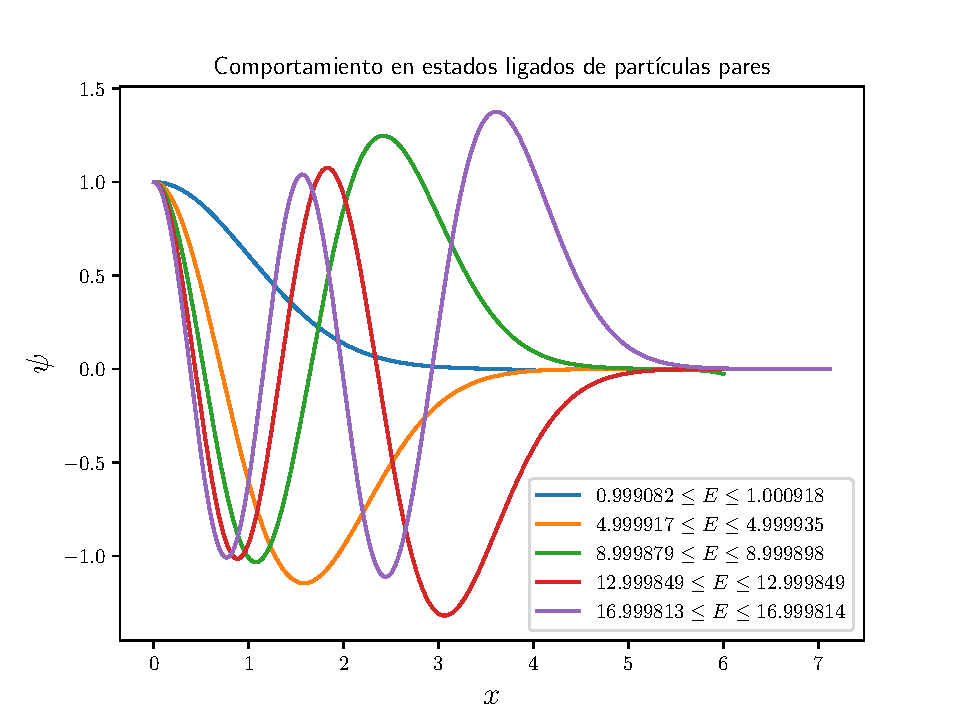
\includegraphics[width = 0.8\textwidth]{comportamiento_ligado_par.pdf}
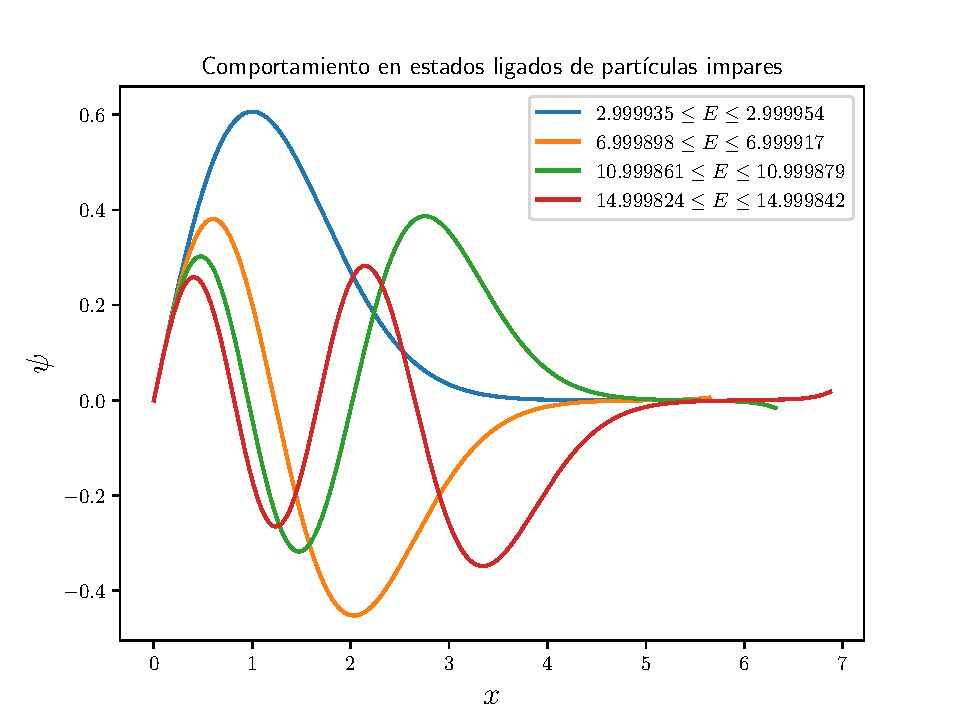
\includegraphics[width = 0.8\textwidth]{comportamiento_ligado_impar.pdf}
\caption{Las soluciones de la funci\'on de onda para una part\'icula en un potencial arm\'onico}
\end{figure}

Es de notar que excepto por el estado base ningun valor de la eneg\'ia se encuentra en el intervalo reportado en la gr\'afica. Esto se debe a la impresici\'on del algoritmo de Euler para resolver ecuaciones diferenciales. En efecto, al momento de aumentar dx (un nombre terrible puesto que normalmente lo que se conoce como "dx" es el tama\~no del intervalo, no la cantidad de intervalos) los intervalos tienden m\'as a las energ\'ias esperadas.

\end{document}
